\documentclass[12pt]{article}
\usepackage[utf8]{inputenc}
\usepackage{graphicx} % Allows you to insert figures
\usepackage{subcaption}
\usepackage{amsmath} % Allows you to do equations
\usepackage{fancyhdr} % Formats the header
\usepackage{geometry} % Formats the paper size, orientation, and margins
\usepackage{dirtytalk} % typesetting different types of quotation
\usepackage[english]{babel}
\usepackage{csquotes}
\usepackage{hyperref}
\usepackage{listings}
\usepackage{xcolor}
\usepackage{array}
\usepackage{caption}
\usepackage{graphicx}  % in preamble
\usepackage{float}     % in preamble, for [H] placement

% % Define code style
% \lstset{
%   basicstyle=\ttfamily\small,
%   backgroundcolor=\color{gray!10},
%   frame=single,
%   breaklines=true,
%   postbreak=\mbox{\textcolor{red}{$\hookrightarrow$}\space},
%   keywordstyle=\color{blue},
%   commentstyle=\color{green!50!black},
%   stringstyle=\color{orange},
% }

% Code styling
\lstset{
    basicstyle=\ttfamily\footnotesize,
    backgroundcolor=\color{lightgray!20},
    keywordstyle=\color{blue},
    commentstyle=\color{green!50!black},
    stringstyle=\color{red},
    numbers=left,
    numberstyle=\tiny\color{gray},
    stepnumber=1,
    numbersep=10pt,
    showspaces=false,
    showstringspaces=false,
    showtabs=false,
    frame=single,
    tabsize=2,
    breaklines=true,
    breakatwhitespace=false,
    escapeinside={\%*}{*)},
    morekeywords={void, size, setup, draw, pushMatrix, popMatrix}
}

\linespread{1.25} % About 1.5 spacing in Word
\setlength{\parindent}{0.8cm} % No paragraph indents
\setlength{\parskip}{0em} % Paragraphs separated by one line
\renewcommand{\headrulewidth}{0pt} % Removes line in header
\geometry{a4paper, portrait, margin=1in}
\setlength{\headheight}{14.49998pt}
\graphicspath{ {images/} }

\begin{document}
\begin{titlepage}
   \begin{center}
    \textsc{\large Ministry of Education of Republic of Moldova}\\[0.5cm]
    \textsc{\large Technical University of Moldova}\\[0.5cm]
    \textsc{\large Faculty of Computers, Informatics and Microelectronics}\\[0.5cm]
    \textsc{\large Department of Physics}\\[1.2cm]
    
    \vspace{25 mm}
    
    \textsc{\Large Criptography and security}\\[0.5cm]
    \textsc{\large Laboratory work \#3}\\[0.5cm]    % <<<<<<< CHANGE LAB NUMBER HERE
    
    \newcommand{\HRule}{\rule{\linewidth}{0.5mm}}
    \vspace{10 mm}
    \HRule \\[0.4cm]
    { \LARGE \bfseries Polyalphabetic ciphers}\\[0.4cm] % <<<<<<< CHANGE LAB TITLE HERE
    \HRule \\[1.5cm]
    
    \vspace{10mm}
    
    \begin{minipage}[t]{0.4\textwidth}
    \begin{flushleft} \large
    \emph{Author:} \\
    Dmitrii \textsc{Belih}\\                         % <<<<<<< CHANGE YOUR NAME HERE
    std. gr. FAF-232                                % <<<<<<< CHANGE GROUP NUMBER HERE
    \end{flushleft}
    \end{minipage}
    ~
    \begin{minipage}[t]{0.4\textwidth}
    \begin{flushright} \large
    \emph{Verified:} \\
    \textsc{Zaica} M.\\
    \end{flushright}
    \end{minipage}\\[3cm]
    
    \vspace{5 mm}
    \large Chișinău 2025\\[0.5cm]
    
    \vfill
    \end{center}
\end{titlepage}

\setcounter{page}{2}
\pagestyle{fancy}
\fancyhf{}
\rhead{\thepage}
\lhead{FAF-232 Belih Dmitrii; Laboratory Work №3s}

\section*{Theory}

The Vigenère Cipher is a method of encrypting alphabetic text that uses a simple form of polyalphabetic substitution. A polyalphabetic cipher is any cipher based on substitution using multiple substitution alphabets. The encryption of the original text is done using the Vigenère square or Vigenère table.

\begin{itemize}
    \item The table consists of the alphabets written out 26 times in different rows, each alphabet shifted cyclically to the left compared to the previous alphabet, corresponding to the 26 possible Caesar Ciphers.
    
    \item At different points in the encryption process, the cipher uses a different alphabet from one of the rows.
    
    \item The alphabet used at each point depends on a repeating keyword.
\end{itemize}

\subsection*{Encryption}

The first letter of the plaintext, G is paired with A, the first letter of the key. So use row G and column A of the Vigenère square, namely G. Similarly, for the second letter of the plaintext, the second letter of the key is used, the letter at row E, and column Y is C. The rest of the plaintext is enciphered in a similar fashion.

\subsection*{Decryption}

Decryption is performed by going to the row in the table corresponding to the key, finding the position of the ciphertext letter in this row, and then using the column's label as the plaintext. For example, in row A (from AYUSH), the ciphertext G appears in column G, which is the first plaintext letter. Next, we go to row Y (from AYUSH), locate the ciphertext C which is found in column E, thus E is the second plaintext letter.

A more easy implementation could be to visualize Vigenère algebraically by converting [A-Z] into numbers [0-25].


\section*{The Task}

Implement the Vigenère algorithm in a single location within the program.

In one place in the program (31 characters), it is possible to specify numbers 0, 1, ... 30. These characters are written in the same way as 'A' to 'Z', 'a' to 'z', and therefore have the correct value range validity. If the user is not satisfied, they can enter other values - and will get the correct value range characters.

The key length must not be smaller than 7. Encryption and decryption will be implemented according to the formula of the most commonly presented mathematical model.

In the message, to eliminate spaces, all letters must be transformed into uppercase. The user will be able to choose the operation - encryption or decryption, will be able to enter the key, the message or cryptogram, and will receive either the cryptogram or the decrypted message.

% \section*{Introduction}
\section*{Technical Implementation}

\subsection*{Class Architecture}
The Vigenère cipher is implemented as a Python class \texttt{VigenereCipher} that encapsulates all cipher functionality.

\subsection*{Alphabet Definition}
\begin{itemize}
    \item Custom 31-character Romanian alphabet: \texttt{"AĂÂBCDEFGHIÎJKLMNOPQRSȘTȚUVWXYZ"}
    \item Alphabet size: 31 characters (indexed 0-30)
    \item Two conversion dictionaries for efficient lookups:
    \begin{itemize}
        \item \texttt{char\_to\_num}: Character → numeric value mapping
        \item \texttt{num\_to\_char}: Numeric value → character mapping
    \end{itemize}
\end{itemize}

\subsection*{Validation Methods}
\subsubsection*{Text Validation}
\begin{verbatim}
def validate_text(self, text):
\end{verbatim}
\begin{itemize}
    \item Checks if input contains only allowed Romanian characters
    \item Allows both uppercase and lowercase letters plus spaces
    \item Returns tuple: (success\_flag, error\_message)
\end{itemize}

\subsubsection*{Key Validation}
\begin{verbatim}
def validate_key(self, key):
\end{verbatim}
\begin{itemize}
    \item Enforces minimum key length of 7 characters
    \item Validates key characters using \texttt{validate\_text()}
    \item Prohibits spaces in the key
    \item Returns tuple: (success\_flag, error\_message)
\end{itemize}

\subsection*{Text Preparation}
\begin{verbatim}
def prepare_text(self, text):
\end{verbatim}
\begin{itemize}
    \item Removes all spaces from input text
    \item Converts all characters to uppercase
    \item Ensures consistent processing format
\end{itemize}

\subsection*{Encryption Algorithm}
\begin{verbatim}
def encrypt(self, plaintext, key):
\end{verbatim}
\begin{enumerate}
    \item Validates both plaintext and key
    \item Prepares text by removing spaces and converting to uppercase
    \item Implements Vigenère formula: 
    \[
    C_i = (P_i + K_i) \mod 31
    \]
    where:
    \begin{itemize}
        \item $C_i$ = ciphertext character at position $i$
        \item $P_i$ = plaintext character numeric value
        \item $K_i$ = key character numeric value ($K_i = key[i \mod key\_length]$)
        \item $31$ = alphabet size
    \end{itemize}
    \item Returns encrypted string and error message
\end{enumerate}

\subsection*{Decryption Algorithm}
\begin{verbatim}
def decrypt(self, ciphertext, key):
\end{verbatim}
\begin{enumerate}
    \item Validates both ciphertext and key
    \item Prepares text by removing spaces and converting to uppercase
    \item Implements inverse Vigenère formula:
    \[
    P_i = (C_i - K_i) \mod 31
    \]
    where:
    \begin{itemize}
        \item $P_i$ = plaintext character at position $i$
        \item $C_i$ = ciphertext character numeric value
        \item $K_i$ = key character numeric value ($K_i = key[i \mod key\_length]$)
        \item $31$ = alphabet size
    \end{itemize}
    \item Returns decrypted string and error message
\end{enumerate}

\subsection*{Helper Functions}
\subsubsection*{Alphabet Table Display}
\begin{verbatim}
def print_alphabet_table(cipher):
\end{verbatim}
\begin{itemize}
    \item Displays the Romanian alphabet with corresponding numeric codes (0-30)
    \item Formats output in two rows for better readability
\end{itemize}

\subsubsection*{Main Program Loop}
\begin{verbatim}
def main():
\end{verbatim}
\begin{itemize}
    \item Interactive menu-driven interface
    \item Four options: Encrypt, Decrypt, Show Alphabet, Exit
    \item Comprehensive error handling and user feedback
    \item Demonstration of usage before main loop execution
\end{itemize}

\subsection*{Key Technical Features}
\begin{itemize}
    \item \textbf{Modular Arithmetic}: Uses modulo 31 operations for the custom alphabet
    \item \textbf{Error Handling}: Comprehensive validation with descriptive error messages
    \item \textbf{Case Insensitivity}: Automatically handles uppercase/lowercase conversion
    \item \textbf{Space Handling}: Removes spaces during processing but maintains readability in UI
    \item \textbf{Key Repeating}: Automatically repeats key using modulo operation for long messages
    \item \textbf{Efficient Lookups}: Uses dictionary mappings for O(1) character conversions
\end{itemize}

\subsection*{Mathematical Model}
The implementation follows the standard Vigenère mathematical model:
\[
Encryption: E(P_i, K_i) = (P_i + K_i) \mod m
\]
\[
Decryption: D(C_i, K_i) = (C_i - K_i) \mod m
\]
Where $m = 31$ (alphabet size), $P_i$ is plaintext character, $C_i$ is ciphertext character, and $K_i$ is key character.

\subsection*{Code Usage Examples}

\subsubsection*{Basic Usage Example}
\begin{verbatim}
# Create cipher instance
cipher = VigenereCipher()

# Define message and key
message = "Bună ziua România"
key = "SECRETKEY"

# Encrypt the message
encrypted, error = cipher.encrypt(message, key)
if encrypted:
    print(f"Encrypted: {encrypted}")

# Decrypt the message
decrypted, error = cipher.decrypt(encrypted, key)
if decrypted:
    print(f"Decrypted: {decrypted}")
\end{verbatim}

\textbf{Output:}
\begin{verbatim}
Encrypted: TȚÎQȚQȚNȚFȚFȚQȚFȚFȚ
Decrypted: BUNAZIUAROMANIA
\end{verbatim}

\subsubsection*{Interactive Program Usage}
\begin{verbatim}
============================================================
VIGENERE CIPHER FOR ROMANIAN LANGUAGE
============================================================

ROMANIAN ALPHABET WITH NUMERIC CODES:
============================================================
A: 0  Ă: 1  Â: 2  B: 3  C: 4  D: 5  E: 6  F: 7  G: 8  H: 9  I:10  Î:11  J:12  K:13  L:14  M:15  
N:16  O:17  P:18  Q:19  R:20  S:21  Ș:22  T:23  Ț:24  U:25  V:26  W:27  X:28  Y:29  Z:30  
============================================================

MENU:
1. Encrypt message
2. Decrypt message
3. Show alphabet
4. Exit

Choose an option (1-4): 1

--- ENCRYPTION ---
Enter the key (min. 7 characters): MYSECRETKEY
Enter message to encrypt: Acesta este un mesaj de test

Original message: Acesta este un mesaj de test
Processed message: ACESTAESTEUNMESAJDETEST
Used key: MYSECRETKEY
Encrypted message: MȚFQȚFȚMQȚFȚMQȚFȚMQȚFȚMQ
\end{verbatim}

\subsubsection*{Error Handling Examples}
\begin{verbatim}
# Example 1: Key too short
key = "SHORT"
encrypted, error = cipher.encrypt("Test message", key)
print(error)  # Output: "The key must have at least 7 characters!"

# Example 2: Invalid characters in message
message = "Hello World!"  # '!' not in Romanian alphabet
encrypted, error = cipher.encrypt(message, "VALIDKEY")
print(error)  # Output: "The character '!' is not allowed..."

# Example 3: Space in key
key = "INVALID KEY"
encrypted, error = cipher.encrypt("Test", key)
print(error)  # Output: "The key cannot contain spaces!"
\end{verbatim}

\subsubsection*{Programmatic Usage}
\begin{verbatim}
# Batch processing multiple messages
cipher = VigenereCipher()
key = "LONGSECRETKEY"

messages = [
    "Primul mesaj important",
    "Al doilea mesaj secret",
    "Ultimul mesaj criptat"
]

for i, message in enumerate(messages, 1):
    encrypted, error = cipher.encrypt(message, key)
    if encrypted:
        print(f"Message {i}: {encrypted}")
        # Verify decryption works
        decrypted, _ = cipher.decrypt(encrypted, key)
        print(f"Decrypted {i}: {decrypted}")
    else:
        print(f"Error with message {i}: {error}")
\end{verbatim}

\subsubsection*{Alphabet Inspection}
\begin{verbatim}
# Display the complete alphabet mapping
cipher = VigenereCipher()
print_alphabet_table(cipher)

# Check specific character mappings
print(f"A -> {cipher.char_to_num['A']}")  # Output: A -> 0
print(f"Ș -> {cipher.char_to_num['Ș']}")  # Output: Ș -> 22
print(f"10 -> {cipher.num_to_char[10]}")  # Output: 10 -> I
print(f"24 -> {cipher.num_to_char[24]}")  # Output: 24 -> Ț
\end{verbatim}

\subsection*{Usage Notes}
\begin{itemize}
    \item The program automatically converts all input to uppercase
    \item Spaces are removed from messages during processing
    \item The key must be at least 7 characters long
    \item Only Romanian alphabet characters are allowed (A-Z, Ă, Â, Î, Ș, Ț)
    \item The same key must be used for encryption and decryption
    \item The interactive program includes built-in usage demonstration
\end{itemize}

    
% \textit{Task1}

% \begin{figure}[h!]
%     \centering
%     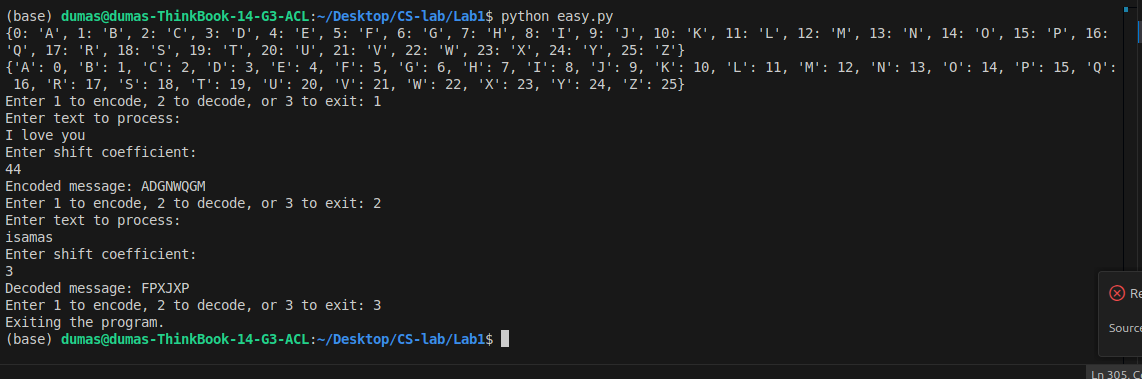
\includegraphics[width=0.8\textwidth]{img/Res1.png}
%     \caption{Result of the encoding and decoding program}
%     \label{fig:result1}
% \end{figure}

% \textit{Task2}

% \begin{figure}[h!]
%     \centering
%     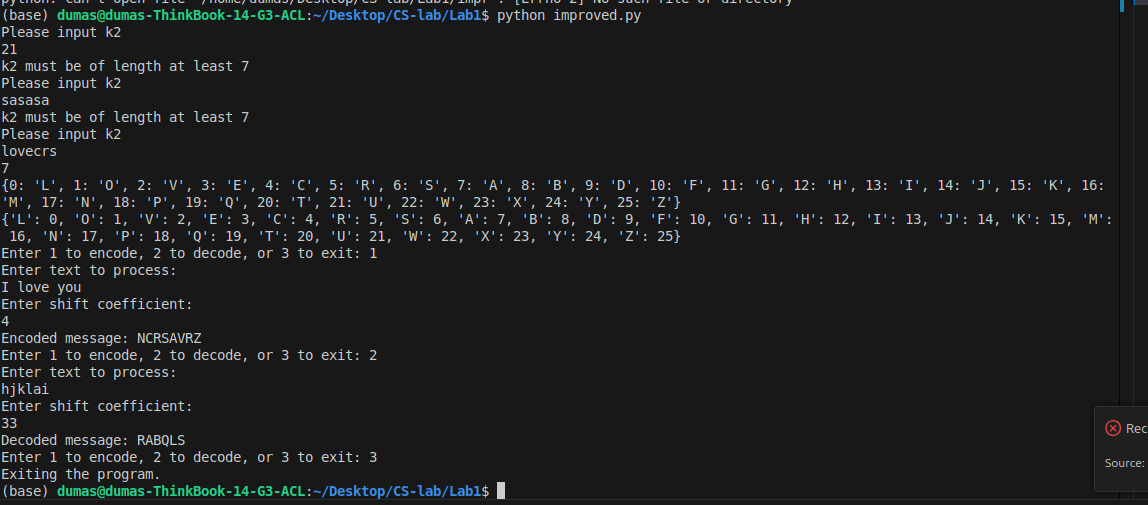
\includegraphics[width=0.8\textwidth]{img/Res2.png}
%     \caption{Result of the encoding and decoding program}
%     \label{fig:result1}
% \end{figure}





\section*{Conclusion}

\hspace{0.8cm}This laboratory work successfully implemented and demonstrated the Vigenère cipher algorithm adapted for the Romanian language with its extended 31-character alphabet. The implementation showcases a robust object-oriented design that encapsulates all cipher functionality within a single Python class, providing both programmatic access for developers and an interactive menu-driven interface for end-users. The cipher correctly applies polyalphabetic substitution principles using modular arithmetic with base 31 to accommodate the specific requirements of the Romanian alphabet.

The implementation meets all specified requirements including the minimum key length of 7 characters, automatic space removal, case normalization, and comprehensive input validation. The mathematical model follows the standard Vigenère formulas for both encryption and decryption operations, ensuring cryptographic correctness. Error handling mechanisms provide clear feedback for invalid inputs while maintaining system stability. The inclusion of both API access and interactive usage makes the implementation versatile for different application scenarios.




\pagebreak
\end{document}